\documentclass[preprint,12pt]{elsarticle}

\usepackage{amssymb}
\usepackage{amsmath}
\usepackage{amsthm}
\usepackage[utf8]{inputenc}
\usepackage{lmodern}
\usepackage{graphicx}
\usepackage{xurl}
\usepackage[hidelinks]{hyperref}

\journal{Discrete Mathematics}

\newcommand{\zenodoID}{10.5281/zenodo.23384809}
\newcommand{\preprintURL}{https://github.com/creelie/didactic-lamp/blob/main/preprintGurvichNaumovaConjecture/GurvichNaumovaConjecture.pdf}

\newtheorem{theorem}{Theorem}[section]
\newtheorem{proposition}[theorem]{Proposition}
\newtheorem{lemma}[theorem]{Lemma}
\newtheorem{corollary}[theorem]{Corollary}
\newtheorem{conjecture}[theorem]{Conjecture}
\theoremstyle{definition}
\newtheorem{definition}[theorem]{Definition}
\newtheorem{remark}[theorem]{Remark}
\newtheorem{example}[theorem]{Example}

\newcommand{\Z}{\mathbb{Z}}
\newcommand{\iv}[2]{[#1,#2]}

\begin{document}

\begin{frontmatter}

\title{Partitioning \texorpdfstring{$\{1,\dots,n\}$}{\{1,...,n\}} into parts of size at most three whose sums are powers of three}

\author[egspl,ucal]{Deep Bhattacharjee\corref{cor1}\fnref{orcid1}}
\ead{itsdeep@live.com}
\ead{d.bhattacharjee@erl-forschung.de}
\fntext[orcid1]{ORCID: \url{https://orcid.org/0000-0003-0466-750X}}
\cortext[cor1]{Corresponding author.}
\affiliation[egspl]{organization={Formerly, Electro-Gravitational Space Propulsion Laboratory (EGSPL)},
            city={Bhubaneswar},
            postcode={751030},
            state={Odisha},
            country={India}}
\affiliation[ucal]{organization={Formerly, University of Calcutta},
            addressline={Senate House, 87/1 College Street},
            city={Kolkata},
            postcode={700073},
            state={West Bengal},
            country={India}}

\author[ntu]{Ushashi Bhattacharya\fnref{orcid2}}
\ead{rai.bhattacharya.in@gmail.com}
\fntext[orcid2]{ORCID: \url{https://orcid.org/0009-0002-2254-3914}}
\affiliation[ntu]{organization={Formerly, National Taiwan University},
            city={Taipei},
            postcode={106319},
            country={Taiwan}}

\begin{abstract}
We prove unconditionally the conjecture of Gurvich and Naumova that for every $n\ge1$ the set $\{1,\dots,n\}$ can be partitioned into parts of at most three elements whose sums are powers of $3$. The partition is given by an explicit recursion.
\end{abstract}

\begin{keyword}
set partition \sep powers of three \sep zero-sum triples \sep formal verification
\MSC[2020] Primary 05A18 \sep Secondary 11B75 \sep 68V15
\end{keyword}

\end{frontmatter}

\section{Introduction}\label{sec:intro}

Let $m\ge2$ and $n\ge1$ be integers and $[n]=\{1,\dots,n\}$. Gurvich and Naumova \cite{GN} call a partition of $[n]$ \emph{$m$-good} if every part has at most $m$ elements and the sum of the elements of every part is a power $m^k$, $k\ge0$, of $m$. Every $[n]$ has exactly one $2$-good partition \cite[Proposition~1]{GN}. In an $m$-good partition every part other than $\{1\}$ has sum $\equiv0\pmod m$, so $n(n+1)/2\equiv0$ or $1\pmod m$. For $n=2(m^t+1)$ this sum is $\equiv3\pmod m$; hence for $m\ge4$ the set $[n]$ has no $m$-good partition \cite[Observation~1]{GN}.\footnote{Partitions of an interval into small parts tied by an additive condition go back to Skolem \cite{Sko57}, who proved that $\{1,\dots,2n\}$ is a disjoint union of pairs $\{a_i,b_i\}$ with $b_i-a_i=i$, $1\le i\le n$, if and only if $n\equiv0$ or $1\pmod4$. Such pairs give a partition of $\{1,\dots,3n\}$ into the $n$ triples $\{i,\,n+a_i,\,n+b_i\}$, each of the form $\{x,y,x+y\}$: the first entries run over $\{1,\dots,n\}$, the other two over $\{n+1,\dots,3n\}$, and $i+(n+a_i)=n+b_i$. In the problem of Gurvich and Naumova the condition is on the sum of a part rather than on a difference.} For $m=3$ they stated:

\begin{conjecture}[{\cite[Conjecture~1]{GN}}]\label{conj:gn}
For every $n\ge1$ the set $[n]$ has a $3$-good partition.
\end{conjecture}

They proved that a minimal counterexample is of the form $n=3^t+3k+2$ with $0\le k<(3^{t-1}-1)/2$ and $k\ne(3^\ell-1)/2$ for $0\le\ell<t$ \cite[Theorem~1]{GN}, recorded further reductions found by O.~Polubasoff, and reported that a computation by D.~Rybin confirmed the conjecture for $n\le844$. We prove it.

\begin{theorem}\label{thm:main}
For every $n\ge1$ the set $[n]$ has a $3$-good partition.
\end{theorem}

\begin{corollary}\label{cor:m}
Let $m\ge2$. Every set $[n]$, $n\ge1$, has an $m$-good partition if and only if $m\in\{2,3\}$.
\end{corollary}

The proof is a recursion on $n$. Let $T=3^t\le n<3T$. For $n=T$, for $2n>3T$, and for $n=T+j$ with $j\not\equiv2\pmod 3$, the reductions of \cite[Section~2]{GN} pass from $[n]$ to a shorter interval. For the remaining $n=T+j$, $j\equiv2\pmod3$, $2j<T$, we prove more: $[n]$ minus the triple $\{n-1,n,T-2j+1\}$, whose sum is $3T$, has a $3$-good partition (Proposition~\ref{prop:H}). This statement passes from $j$ to $n$ by a reflection argument (Lemma~\ref{lem:assembly}), except when $j$ lies in the upper half of the interval $[3^u,3^{u+1})$ that contains it. In that case a fixed-point-free involution of $\{1,\dots,2N-2\}$ with distinct pair sums supplies the missing triples (Lemma~\ref{lem:sigma}). Figure~\ref{fig:cases} shows the four cases, and Section~\ref{sec:lean} describes the formal verification of the proof.

\begin{figure}[t]
\centering
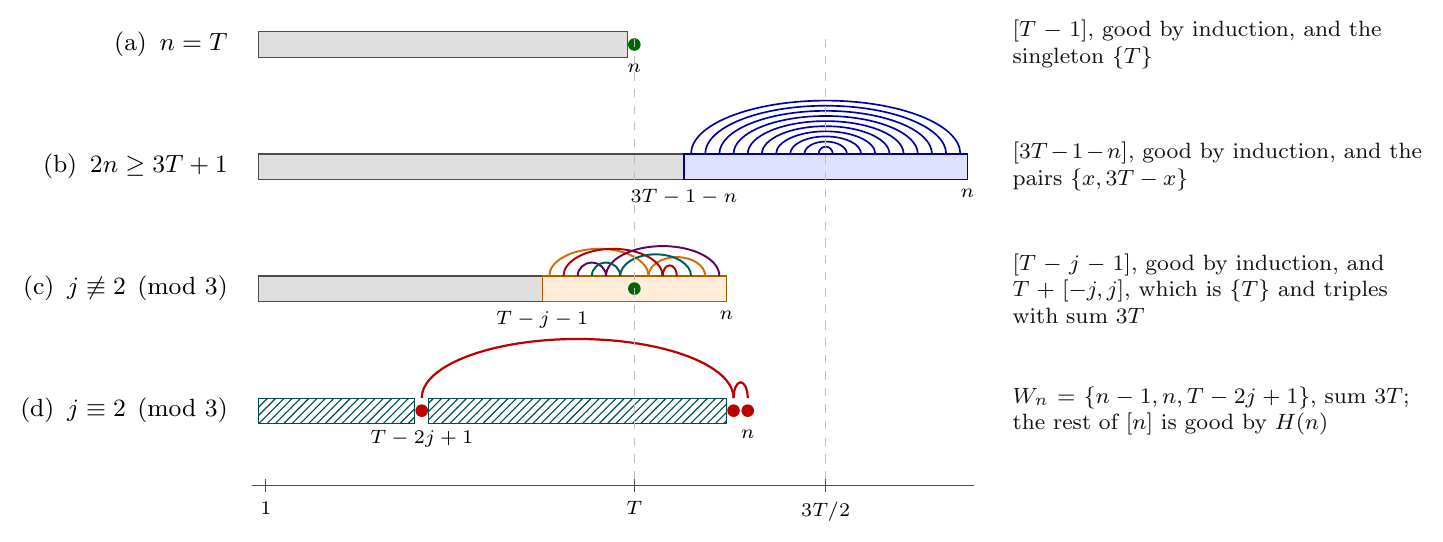
\includegraphics[width=\textwidth]{figures/fig_cases.png}
\caption{The four cases of the recursion for $T=27$, drawn for $n=27,50,33,35$. In (a)--(c) the gray interval is good by induction. In (d) the three red points form $W_n$, and the rest of $[n]$ is good by $H(n)$, Proposition~\ref{prop:H}.}\label{fig:cases}
\end{figure}

\section{Good and balanced sets}\label{sec:prelim}

For integers $a\le b$ let $\iv ab=\{x\in\Z: a\le x\le b\}$, and $\iv ab=\emptyset$ if $a>b$. For $Z\subset\Z$ and $c,s\in\Z$ write $c+sZ=\{c+sz:z\in Z\}$ and $c-Z=\{c-z:z\in Z\}$. A finite set $A\subset\Z$ is \emph{admissible} if $|A|\le3$ and $\sum_{x\in A}x=3^k$ for some $k\ge0$. A finite set $S\subset\Z$ is \emph{good} if it is a disjoint union of admissible sets;\footnote{A partition of $S$ is a cover of $S$ in which every point lies in exactly one set. Covers in which every point lies in at least $k$ of the sets, and the nerve complexes that record how the sets of a cover meet, are studied in~\cite{BB26}.} thus $[n]$ is good if and only if it has a $3$-good partition. A finite set $Z\subset\Z$ is \emph{balanced} if it is a disjoint union of sets each of which is $\{0\}$ or a $3$-element set with sum $0$. Disjoint unions of good sets are good, and disjoint unions of balanced sets are balanced.

\begin{lemma}[{\cite[Lemma~1]{GN}}]\label{lem:interval}
If $\ell\ge0$ and $\ell\not\equiv2\pmod3$, then $\iv{-\ell}{\ell}$ is balanced.
\end{lemma}

\begin{proof}
Write $\ell=3k+r$ with $r\in\{0,1\}$. For $0\le i<k$ the sets
\[
A_i=\{-(3k-i),\,1+i,\,3k-1-2i\},\qquad B_i=\{-(2k-i),\,-(k-i),\,3k-2i\}
\]
have sum $0$. As $i$ runs over $\iv0{k-1}$, the entries $-(3k-i)$, $-(2k-i)$, $-(k-i)$ run over $\iv{-3k}{-2k-1}$, $\iv{-2k}{-k-1}$, $\iv{-k}{-1}$, the entries $1+i$ run over $\iv1k$, and the entries $3k-1-2i$ and $3k-2i$ run over the numbers in $\iv{k+1}{3k}$ of the parity of $3k-1$ and of $3k$. So the $2k$ sets $A_i,B_i$ partition $\iv{-3k}{3k}\setminus\{0\}$. Add $\{0\}$ if $r=0$ and $\{-\ell,0,\ell\}$ if $r=1$.
\end{proof}

In \cite{GN} the index $i$ runs from $1$; it has to start at $0$, as the examples $k=1,2$ given there show.

\begin{lemma}\label{lem:image}
Let $Z$ be balanced, $q\ge0$ and $s\ne0$. Then $3^q+sZ$ is good and $sZ$ is balanced.
\end{lemma}

\begin{proof}
The map $x\mapsto 3^q+sx$ is injective; it sends $\{0\}$ to $\{3^q\}$ and a $3$-element set with sum $0$ to a $3$-element set with sum $3^{q+1}$. The map $x\mapsto sx$ is injective and preserves the two kinds of parts.
\end{proof}

\begin{lemma}\label{lem:pairs}
Let $Q=3^q$ and let $X\subseteq\iv1{Q-1}$ satisfy $Q-X=X$. Then $X$ is good.
\end{lemma}

\begin{proof}
Since $Q$ is odd, $x\ne Q-x$, and $X$ is the disjoint union of the pairs $\{x,Q-x\}$ with $x\in X$, $x<Q/2$; each has sum $Q$.
\end{proof}

\section{Reflection and the involutions \texorpdfstring{$\sigma_N$}{sigma\_N}}\label{sec:tools}

The next lemma uses the reflection $x\mapsto T-x$ of $\iv1{T-1}$, an action of the group of order two that pairs off the points of a symmetric set.\footnote{For an action of a group $G$ on a set, the orbits of $G$ partition the set; here $G$ has order two and the orbits are the pairs $\{x,T-x\}$, all of size two because $T$ is odd. Equivariant classes for actions of hyperbolic groups are constructed in~\cite{Bha22}.}

\begin{lemma}\label{lem:assembly}
Let $T=3^t$, $j\ge0$, $D\subseteq\iv1{T-1}$ and $W\subseteq\iv{T+1}{T+j}\cup(T-D)$. Put
\[
F=\{d\in D:T-d\notin D\},\qquad R=\bigl(\{T\}\cup\iv{T+1}{T+j}\cup(T-D)\bigr)\setminus W.
\]
If $F$ and $R$ are good, then $\iv1{T+j}\setminus W$ is good.
\end{lemma}

\begin{proof}
Let $E=\{x\in\iv1{T-1}: x\notin D,\ T-x\notin D\}$. Then $T-E=E$, so $E$ is good by Lemma~\ref{lem:pairs}. We show that $\iv1{T+j}\setminus W$ is the disjoint union of $E$, $F$ and $R$. The set $E$ meets neither $D\supseteq F$ nor $\{T\}\cup\iv{T+1}{T+j}\cup(T-D)\supseteq R$; and $F\subseteq\iv1{T-1}$ does not meet $T-D$, hence meets neither $R$ nor $W$. Since $E$ does not meet $W$ either, $E$, $F$, $R$ are disjoint subsets of $\iv1{T+j}\setminus W$. Conversely let $x\in\iv1{T+j}\setminus W$. If $x\ge T$, or if $x\le T-1$ and $T-x\in D$, then $x\in R$. Otherwise $x\le T-1$, $T-x\notin D$, and $x\in F$ or $x\in E$ according as $x\in D$ or not.
\end{proof}

\begin{figure}[t]
\centering
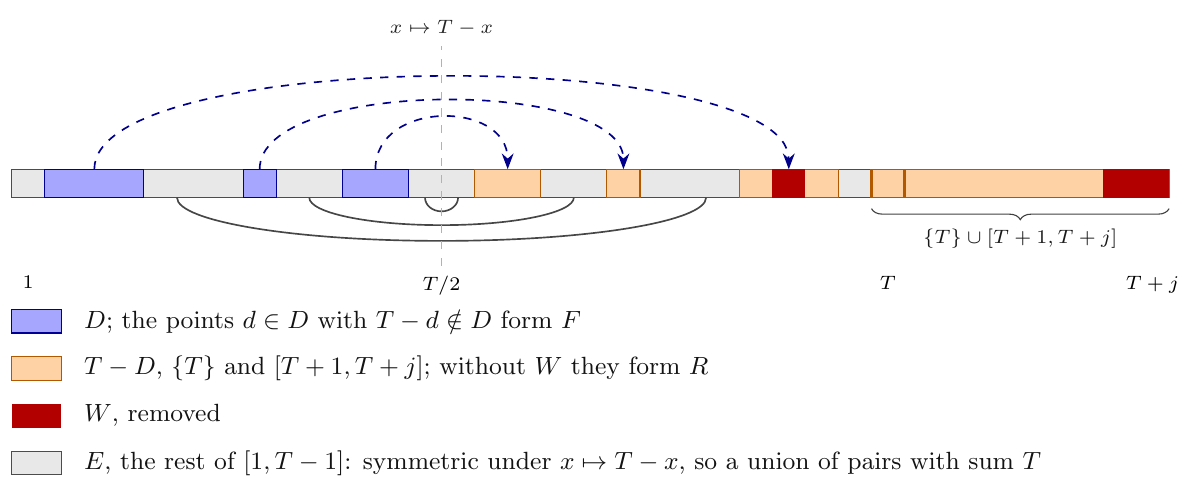
\includegraphics[width=\textwidth]{figures/fig_assembly.png}
\caption{Lemma~\ref{lem:assembly}. The reflection $x\mapsto T-x$ maps $D$ onto $T-D$; the rest $E$ of $\iv1{T-1}$ is symmetric and splits into pairs with sum $T$.}\label{fig:assembly}
\end{figure}

\begin{lemma}\label{lem:sigma}
Let $N\ge1$, $N\equiv1\pmod3$, and $K=2N-2$. There is a fixed-point-free involution\footnote{A fixed-point-free involution is a free action of the group of order two, and its orbits are pairs. On complex surfaces the same notion gives the Enriques surfaces, which are the quotients of K3 surfaces by fixed-point-free involutions; K3 surfaces with involutions and the Enriques and Kummer surfaces obtained from them are studied in~\cite{BN26}.} $\sigma$ of $\iv1K$ with the following properties, where $\Pi=\{z\in\iv1K:z<\sigma(z)\}$.
\begin{enumerate}
\item[(i)] The sums $z+\sigma(z)$, $z\in\Pi$, are distinct.
\item[(ii)] The $N$ numbers $2N-2$ and $z+\sigma(z)-(2N+1)$, $z\in\Pi$, are distinct, and the set $\Delta_N$ they form is balanced.
\item[(iii)] Every $\delta\in\Delta_N$ satisfies $|\delta|\le 2N-2$, and every positive $\delta\in\Delta_N$ is even.
\end{enumerate}
\end{lemma}

\begin{proof}
Since $N\equiv1\pmod3$, either $N=1$, or $N=2M$ with $M\ge2$ and $M\equiv2\pmod3$, or $N=2M+1$ with $M\ge3$ and $M\equiv0\pmod3$.

If $N=1$, then $\iv1K=\emptyset$ and $\Delta_1=\{0\}$.

Let $N=2M$. Let $\sigma$ exchange $z\leftrightarrow z+N-1$ for $1\le z\le N-1$. These pairs partition $\iv1K$, since $K=2(N-1)$. The pair sums are $2z+N-1$, $1\le z\le N-1$, which are distinct. Subtracting $2N+1=4M+1$ gives the numbers $2(z-M-1)$, $1\le z\le 2M-1$, so $\Delta_N=\{4M-2\}\cup2\,\iv{-M}{M-2}$, that is,
\[
\Delta_N=\{4M-2,\,-2M,\,-(2M-2)\}\cup 2\,\iv{-(M-2)}{M-2}.
\]
The first set has sum $0$; the second lies in $\iv{-(2M-4)}{2M-4}$, so it does not meet the first, and it is balanced by Lemmas~\ref{lem:interval} and~\ref{lem:image}, since $M-2\equiv0\pmod3$. This proves (i)--(iii), as $4M-2=2N-2$.

Let $N=2M+1$. Let $\sigma$ exchange $1\leftrightarrow N$, $2\leftrightarrow N+1$, $3\leftrightarrow N-1$, $4\leftrightarrow N+2$, $2N-3\leftrightarrow2N-2$, and $x\leftrightarrow x+N-2$ for $5\le x\le N-2$. The last family pairs $\iv5{N-2}$ with $\iv{N+3}{2N-4}$, so these pairs partition $\iv1K$. The pair sums are $N+1$, $N+3$, $N+2$, $N+6$, $4N-5$ and $2x+N-2\in\iv{N+8}{3N-6}$, $5\le x\le N-2$, which are distinct. Subtracting $2N+1=4M+3$ gives
\begin{multline*}
\Delta_N=\{4M,\,-(2M+1),\,-(2M-1)\}\cup\{4M-4,\,-2M,\,-(2M-4)\}\\
\cup 2\,\iv{-(M-3)}{M-3}.
\end{multline*}
The first two sets have sum $0$; the third lies in $\iv{-(2M-6)}{2M-6}$ and is balanced since $M-3\equiv0\pmod3$. The three sets are disjoint, which proves (i)--(iii), as $4M=2N-2$.
\end{proof}

\begin{figure}[t]
\centering
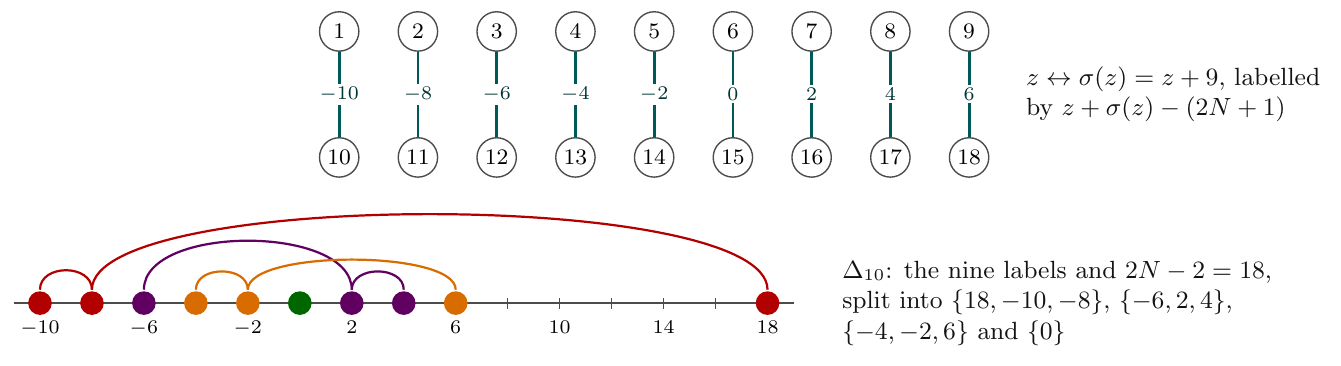
\includegraphics[width=0.92\textwidth]{figures/fig_sigma.png}
\caption{Lemma~\ref{lem:sigma} for $N=10$, $M=5$. Each pair $\{z,\sigma(z)\}$ carries the number $z+\sigma(z)-(2N+1)$; together with $2N-2=18$ these form $\Delta_{10}$, which splits into three triples with sum $0$ and $\{0\}$.}\label{fig:sigma}
\end{figure}

\section{Proof of \texorpdfstring{Theorem~\ref{thm:main}}{the theorem}}\label{sec:proof}

For $n\ge1$ let $t$ be the integer with $3^t\le n<3^{t+1}$. If $t\ge1$ and $j=n-3^t$ satisfies
\begin{equation}\label{eq:range}
j\equiv2\pmod3,\qquad 2\le j,\qquad 2j+1\le3^t,
\end{equation}
put $W_n=\{n-1,\,n,\,3^t-2j+1\}$. Its elements are distinct, since $2\le 3^t-2j+1\le3^t-3$, and their sum is $3^{t+1}$. Let $H(n)$ be the statement that $[n]\setminus W_n$ is good.

\begin{proposition}\label{prop:H}
Let $n=3^t+j$ with $t\ge1$ and $j$ as in \eqref{eq:range}. Suppose that $[m]$ is good for every $m<n$ and that $H(m)$ holds for every $m<n$ for which it is defined. Then $H(n)$ holds.
\end{proposition}

\begin{proof}
Let $T=3^t$, so $W_n=\{T+j-1,T+j,T-2j+1\}$. Since $T\ge2j+1\ge5$, we have $T\ge9$. In each case below we choose $D\subseteq\iv1{T-1}$ with $2j-1\in D$, so that $W=W_n\subseteq\iv{T+1}{T+j}\cup(T-D)$, and show that the sets $F$ and $R$ of Lemma~\ref{lem:assembly} are good. Lemma~\ref{lem:assembly} then gives $H(n)$.

\emph{Case $j=2$.} Take $D=\{3\}$. Then $F=\{3\}$, as $T-3\ne3$, and $R=\{T,T+1,T+2,T-3\}\setminus W=\{T\}$.

For $j\ge5$ let $u$ be the integer with $3^u\le j<3^{u+1}$. Then $u\ge1$, and $j\ge3^u+2$ because $j\equiv2$ and $3^u\equiv0\pmod 3$. Also $3j\ne T$, since $3j=T$ would give $j=3^{t-1}\equiv0\pmod3$.

\emph{Cases $3j>T$, and $3j<T$ with $2j+1\le3^{u+1}$.} Take $D=\iv1{j-2}\cup\{2j-1\}$. Then $T-D=\iv{T-j+2}{T-1}\cup\{T-2j+1\}$ and
\[
R=T+\iv{-(j-2)}{j-2},
\]
which is good by Lemmas~\ref{lem:interval} and~\ref{lem:image}, since $j-2\equiv0\pmod3$.

If $3j>T$, then $u=t-1$. As $T$ and $3j$ are multiples of $3$, $T\le3j-3$, so $T-2j+1\in\iv2{j-2}\subseteq D$. For $d\in\iv1{j-2}$ we have $T-d\ge T-j+2>j-2$, so $T-d\in D$ only if $T-d=2j-1$. Hence
\[
F=\iv1{j-2}\setminus\{T-2j+1\}=[j]\setminus W_j,
\]
because $3^{u+1}=T$ and $W_j=\{j-1,j,T-2j+1\}$. The number $j=3^u+(j-3^u)$ satisfies \eqref{eq:range} at level $u$, so $F$ is good by $H(j)$.

If $3j<T$ and $2j+1\le3^{u+1}$, then $3^{u+1}\le3j<T$ gives $T\ge3^{u+2}$, and every $d\in D$ satisfies $T-d\ge T-2j+1>3^{u+2}-3^{u+1}>2j-1$. Hence $F=D$. Put $p=3^{u+1}-2j+1$; then $2\le p\le j-2$, because $2j+1\le 3^{u+1}$ and $j\ge3^u+1$. Since $W_j=\{j-1,j,p\}$,
\[
F=D=\bigl([j]\setminus W_j\bigr)\cup\{p,\,2j-1\},
\]
a disjoint union of a set that is good by $H(j)$ and a pair with sum $3^{u+1}$.

\emph{Case $3j<T$ and $2j+1>3^{u+1}$.} Let $P=3^{u+1}$. As before $T\ge3P$, so $T=3P$ or $T\ge9P$; and $P+1\le2j\le2P-2$. Write $P=2c+1$ and put
\[
N=j-c,\qquad e=P-1-j=c-N.
\]
Then $N\ge1$, $e\ge0$, $j=e+2N$, and $2N-2=2j-P-1\le P-3$. Since $3\mid P$ we have $c\equiv1\pmod3$, hence $N\equiv1$ and $e\equiv0\pmod 3$. Let $\sigma$, $\Pi$, $\Delta_N$ be as in Lemma~\ref{lem:sigma}, $K=2N-2$, and
\[
D=\iv1e\cup(P+\Delta_N).
\]
By Lemma~\ref{lem:sigma}(iii), $P+\Delta_N\subseteq\iv{P-2N+2}{P+2N-2}=\iv{2e+3}{2j-1}$, so the union is disjoint, $D\subseteq\iv1{2P-3}\subseteq\iv1{T-1}$, and $2j-1=P+(2N-2)\in D$.

We show $F=D$. Let $d,d'\in D$ with $d+d'=T$. If $d\le e$, then $d+d'\le e+2P-3<3P\le T$; so $d=P+\delta$ and $d'=P+\delta'$ with $\delta,\delta'\in\Delta_N$ and $\delta+\delta'=T-2P$. If $T\ge9P$, then $\delta+\delta'\ge7P>2(P-3)$, which is impossible. If $T=3P$, then $\delta+\delta'=P$ is odd. Since $\delta,\delta'\le P-3$, both are positive, hence even by Lemma~\ref{lem:sigma}(iii), a contradiction. Thus $F=D$, which is good: $\iv1e=[e]$ is good by hypothesis, and $P+\Delta_N$ by Lemmas~\ref{lem:sigma} and~\ref{lem:image}.

It remains to compute $R$. First, $\iv{T+1}{T+j}\setminus W=T+\iv1{j-2}=T+\iv1{e+K}$. Second, $T-D=T+\iv{-e}{-1}$ together with $T-P-\Delta_N$; here $T-P-(2N-2)=T-2j+1\in W$, and for $z\in\Pi$, using $P-2N-1=2e$,
\[
T-P-\bigl(z+\sigma(z)-(2N+1)\bigr)=T-\bigl(2e+z+\sigma(z)\bigr).
\]
By Lemma~\ref{lem:sigma}(ii) these numbers differ from $T-2j+1$. Hence $R=T+Z$ with
\[
Z=\iv{-e}{e}\ \cup\bigcup_{z\in\Pi}\bigl\{e+z,\ e+\sigma(z),\ -(2e+z+\sigma(z))\bigr\}.
\]
Each set $\{e+z,e+\sigma(z),-(2e+z+\sigma(z))\}$ has three elements and sum $0$. As $z$ runs over $\Pi$, the numbers $e+z$ and $e+\sigma(z)$ run over $e+\iv1K$ once each, because $\sigma$ is a fixed-point-free involution; the numbers $-(2e+z+\sigma(z))$ are distinct by Lemma~\ref{lem:sigma}(i) and less than $-e$. Since $\iv{-e}{e}$ is balanced by Lemma~\ref{lem:interval}, $Z$ is balanced, and $R$ is good by Lemma~\ref{lem:image}.
\end{proof}

\begin{proof}[Proof of Theorem~\ref{thm:main}]
We prove by strong induction on $n\ge0$ that $[n]$ is good and that $H(n)$ holds whenever it is defined; $[0]=\emptyset$. The sets $[1]=\{1\}$ and $[2]=\{1,2\}$ are admissible, and $H(1)$, $H(2)$ are not defined. Let $n\ge3$, $T=3^t\le n<3T$, $t\ge1$. Whenever $H(n)$ is defined, it holds by Proposition~\ref{prop:H} and the induction hypothesis. For $[n]$ there are four cases.
\begin{enumerate}
\item[(a)] $n=T$: $[n]=[T-1]\cup\{T\}$.
\item[(b)] $2n\ge3T+1$: with $a=3T-1-n<n$, $[n]=[a]\cup\iv{a+1}{3T-1-a}$, and the second set is good by Lemma~\ref{lem:pairs} with $Q=3T$.
\item[(c)] $T<n$, $2n\le3T$ and $j=n-T\not\equiv2\pmod3$: $[n]$ is the union of $[T-j-1]$ and $T+\iv{-j}{j}$, and the second set is good by Lemmas~\ref{lem:interval} and~\ref{lem:image}.
\item[(d)] $T<n$, $2n\le3T$ and $j=n-T\equiv2\pmod3$: then $j$ satisfies \eqref{eq:range}, and $[n]=([n]\setminus W_n)\cup W_n$, where $[n]\setminus W_n$ is good by $H(n)$ and $W_n$ is admissible.
\end{enumerate}
In (a)--(c) the first set is good by the induction hypothesis, and in all cases the union is disjoint.
\end{proof}

\begin{proof}[Proof of Corollary~\ref{cor:m}]
For $m=2$ this is \cite[Proposition~1]{GN}, for $m=3$ it is Theorem~\ref{thm:main}, and for $m\ge4$ the set $[2m+2]$ has no $m$-good partition, as recalled in Section~\ref{sec:intro}.
\end{proof}

\begin{example}\label{ex:35}
The least $n$ not excluded by \cite[Theorem~1]{GN} is $n=35=27+8$. Here $3j=24<27$, $u=1$ and $2j+1=17>9$, so the last case applies with $P=9$, $c=4$, $N=4$, $e=0$. The involution $\sigma$ of $\iv16$ is $1\leftrightarrow4$, $2\leftrightarrow5$, $3\leftrightarrow6$, $\Delta_4=\{6,-4,-2,0\}$ and $D=\{5,7,9,15\}$. The construction gives the $3$-good partition of $[35]$ into
\[
\{5,7,15\},\ \{9\},\ \{27\},\ \{18,30,33\},\ \{20,29,32\},\ \{22,28,31\},\ \{12,34,35\}
\]
and the nine pairs $\{x,27-x\}$, $x\in\{1,2,3,4,6,8,10,11,13\}$; see Figure~\ref{fig:example}.
\end{example}

\begin{figure}[t]
\centering
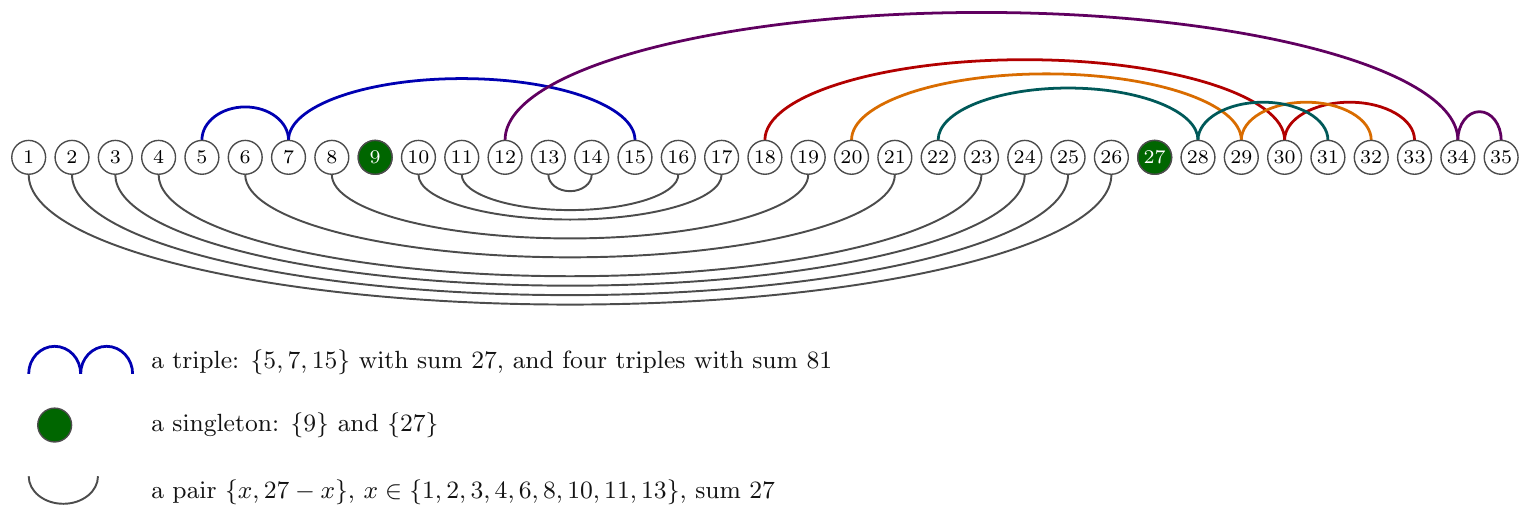
\includegraphics[width=\textwidth]{figures/fig_example.png}
\caption{The $3$-good partition of $[35]$ given by the recursion. Each triple is drawn as two arcs above the line, each pair as one arc below it.}\label{fig:example}
\end{figure}

The recursion computes the partition of $[n]$ in $O(n)$ arithmetic operations.

\section{Formal verification}\label{sec:lean}

Theorem~\ref{thm:main} is formalized in Lean~4 \cite{MU21} with Mathlib \cite{Mathlib20}, version~4.34.1, and the formal proof is checked by the Lean kernel. The formal statement says that for every natural number $n$ there is a partition of $\{1,\dots,n\}$ into nonempty parts, each of which has at most three elements and a power of $3$ as its sum. In the formal proof, good and balanced sets are the finite sets of integers built by disjoint union from the admissible sets, respectively from $\{0\}$ and the $3$-element sets with sum $0$, and the argument is that of Sections~\ref{sec:prelim}--\ref{sec:proof}. The proof depends only on the axioms of Lean's logic, namely propositional extensionality, choice and the soundness of quotients; it has no unproved step and adds no axiom.

Independent computations in exact integer arithmetic run the recursion of Section~\ref{sec:proof} and confirm that it gives a $3$-good partition of $[n]$ for every $n\le30000$ and for further values of $n$ up to $6.5\cdot10^7$, and that $H(n)$ holds for every $n$ in these ranges for which it is defined. They also confirm Lemma~\ref{lem:interval} for $\ell\le30000$ and Lemma~\ref{lem:sigma} for $N\le30001$.

\section*{Data and code availability}
\begingroup\raggedright
The \LaTeX{} source of the paper, the Lean~4 formalization of Theorem~\ref{thm:main} and the programs of Section~\ref{sec:lean} are archived at Zenodo under doi:\href{https://doi.org/\zenodoID}{\zenodoID} \cite{archive}; the paper is available at \url{\preprintURL}. Deep Bhattacharjee carried out the computations and the Lean, Julia, C, C\texttt{++}, Python and shell verifications, and the proofs and the text were drafted, with AI assistance (Claude, Anthropic); both authors approved the final version.\par
\endgroup

\section*{Ethical declarations}
Funding: none. Competing interests: none.

\begin{thebibliography}{9}
\raggedright
\expandafter\ifx\csname url\endcsname\relax
  \def\url#1{\texttt{#1}}\fi
\expandafter\ifx\csname urlprefix\endcsname\relax\def\urlprefix{URL }\fi
\expandafter\ifx\csname href\endcsname\relax
  \def\href#1#2{#2} \def\path#1{#1}\fi

\bibitem{GN}
V.~Gurvich, M.~Naumova, Partitioning set $[n]=\{1,\dots,n\}$ into subsets of size at most $m$ such that all sums are powers of $m$, arXiv:2508.00946 [math.CO] (2025).
\newblock \href {https://doi.org/10.48550/arXiv.2508.00946}
  {\path{doi:10.48550/arXiv.2508.00946}}.

\bibitem{Sko57}
Th.~Skolem, On certain distributions of integers in pairs with given differences, Math. Scand. 5 (1957) 57--68.
\newblock \href {https://doi.org/10.7146/math.scand.a-10490}
  {\path{doi:10.7146/math.scand.a-10490}}.

\bibitem{MU21}
L.~de~Moura, S.~Ullrich, The {L}ean 4 theorem prover and programming language,
  in: Automated Deduction -- CADE 28, Vol. 12699 of Lecture Notes in Comput.
  Sci., Springer, Cham, 2021, pp. 625--635.
\newblock \href {https://doi.org/10.1007/978-3-030-79876-5_37}
  {\path{doi:10.1007/978-3-030-79876-5_37}}.

\bibitem{Mathlib20}
{The mathlib Community}, The {L}ean mathematical library, in: Proceedings of
  the 9th ACM SIGPLAN International Conference on Certified Programs and
  Proofs, ACM, New York, 2020, pp. 367--381.
\newblock \href {https://doi.org/10.1145/3372885.3373824}
  {\path{doi:10.1145/3372885.3373824}}.

\bibitem{BB26}
D.~Bhattacharjee, U.~Bhattacharya, Iterated nerve complexes for $k$-fold sensor coverage, Preprints.org (2026).
\newblock \href {https://doi.org/10.20944/preprints202606.1351.v2}
  {\path{doi:10.20944/preprints202606.1351.v2}}.

\bibitem{Bha22}
D.~Bhattacharjee, Establishing equivariant class $[O]$ for hyperbolic groups, Asian Res. J. Math. 18~(11) (2022) 362--369.
\newblock \href {https://doi.org/10.9734/arjom/2022/v18i11615}
  {\path{doi:10.9734/arjom/2022/v18i11615}}.

\bibitem{BN26}
D.~Bhattacharjee, P.~Nandi, Enriques and {K}ummer surfaces arising from {K3} involutions, Preprints.org (2026).
\newblock \href {https://doi.org/10.20944/preprints202602.0098.v1}
  {\path{doi:10.20944/preprints202602.0098.v1}}.

\bibitem{archive}
D.~Bhattacharjee, U.~Bhattacharya, Partitioning $\{1,\dots,n\}$ into parts of size at most three whose sums are powers of three: paper, Lean 4 formalization and verification code, Zenodo (2026).
\newblock \href {https://doi.org/10.5281/zenodo.23384809}
  {\path{doi:10.5281/zenodo.23384809}}.

\end{thebibliography}

\end{document}
